\RequirePackage{xcolor}
\documentclass[shortabstract, manyadvisors, english, mgr]{iithesis}
\usepackage[utf8]{inputenc}
\usepackage{minted, fancyvrb, epigraph, xurl, pifont, graphicx}

\englishtitle{Implementation of the Terminal Subsystem \\ and Job Control \\
  in the Mimiker Operating System}
\polishtitle{Implementacja podsystemu terminali i kontroli zadań \\
  w systemie operacyjnym Mimiker}

\englishabstract{English Abstract}
\polishabstract{Polish Abstract}
\author{Jakub Piecuch}
\advisor{Krystian Bacławski \fmlinebreak Piotr Witkowski}

% \date{} % Data zlozenia pracy

\transcriptnum{281940}

\makeatletter
\minted@def@optcl@switch{stdlibhighlighting}{-P stdlibhighlighting}
\minted@def@optcl@switch{c99highlighting}{-P c99highlighting}
\minted@def@optcl@switch{c11highlighting}{-P c11highlighting}
\minted@def@optcl@switch{platformhighlighting}{-P platformhighlighting}
\AtBeginDocument{%
  \newcounter{llabel}[listing]%
  \renewcommand*{\thellabel}{%
    \ifnum\value{llabel}<0 %
      \@ctrerr
    \else
      \ifnum\value{llabel}>10 %
        \@ctrerr
      \else
        \protect\ding{\the\numexpr\value{llabel}+201\relax}%
      \fi
    \fi
  }%
}
\newlength{\llabelsep}
\setlength{\llabelsep}{1pt}
\newcommand*{\llabel}[1]{%
  \begingroup
  \refstepcounter{llabel}%
  \label{#1}%
  \llap{\thellabel\kern\llabelsep}%
  \endgroup
}
\makeatother

\setminted[c]{fontsize=\small, frame=lines, baselinestretch=1.1, stdlibhighlighting=false,
  c99highlighting=false, c11highlighting=false, platformhighlighting=false, escapeinside=@@}

\renewcommand\linenumberfont{\normalfont\bfseries\large}
%\renewcommand{\theFancyVerbLine}{\arabic{FancyVerbLine}}

\begin{document}

\chapter{Introduction}

XXX nie jestem jeszcze pewien jak powinno wyglądać wprowadzenie. Zabiorę się za
nie jako ostatnie. To co jest teraz napisane prawdopodobnie wyrzucę, ale
zostawiam do wglądu.

POMYSŁ NA WPROWADZENIE:
\begin{itemize}
\item Przedstawienie kontroli zadań w powłoce (motywacja).
\item Jakie rzeczy są potrzebne żeby to wszystko działało? Sygnały, grupy
  procesów itp.
\item W Mimikerze to nie działało, a teraz działa, i o tym jest ta praca.
\end{itemize}

\section{What is a terminal?}

\subsection{Early-day terminals}

In the early days of computing, a computer had a single operator. Users would
submit their programs to the operator, usually on punched cards. When the user's
turn came, the operator would load the program into the machine, and collect the
output of the program in the form of punched cards. The whole process usually
took hours. If the program contained an error, the user would know about it no
sooner than when the operator loads it into the machine. Clearly, a more
interactive way of submitting programs for execution was needed.

Time-sharing systems were the solution to this problem. A time-sharing system
allows users to interact with the machine using a terminal. It gives the user an
illusion of exclusive posession of the machine's resources. In reality, the
operating system provides a fraction of the machine's computing resources to
each user. Multics\cite{multics} is an early example of a time-sharing operating
system.

In general, a terminal device is any device that allows its user to interact
with a computing system, such as a mainframe. It allows the user to input
commands, data, or even whole programs, and to examine the system's output.
A terminal could communicate with the system remotely, or be directly attached
to it.

In the beginning, terminals were electromechanical teletypewriters
(teletypes, or TTYs for short), initially used in telegraphy. A teletype
sends data typed on the keyboard to the computer, and prints the response.

In the 1970, video terminals came into widespread use. A video terminal displays
output on a screen instead of printing it. Most models provide a set of special
\textit{escape codes}: sequences of characters that, when sent to the terminal,
cause some action, e.g. clearing the screen. One of the most common features is
a cursor that can be controlled using escape codes. This made tasks such as
editing text much more enjoyable. The DEC VT100 series of video terminals was
extremely successful, and is the basis of a de facto standard for terminal
escape codes.

\subsection{Terminals in a modern context}

Nowadays, most people use their computer via a graphical user interface, or GUI.
There is no dedicated device that handles interaction between the system and the
user: input can be provided and output can be displayed by multiple devices. For
instance, user input can be provided by a combination of a keyboard and mouse,
and output can be displayed on a pair of monitors. Consequently, input and
output handling in GUI programs is considerably more complex compared to
programs written for character-based terminals. In addition, some people simply
prefer to use a text-based, non-graphical interface due to its efficiency. For
these reasons, it is useful to provide a means to run programs that use a
terminal-based interface. This is accomplished using a \textit{terminal
emulator}.

A terminal emulator is a GUI program that emulates a terminal device, usually
one that is compatible with the VT100 series of video terminals. The display of
the emulated terminal is presented in the emulator's GUI window. The emulator
translates the user's keystrokes into characters and feeds them as input to the
application running inside the emulator. Output from the application is
displayed in the GUI window in the same way it would be displayed on a real
video terminal's screen. \texttt{xterm} is an example of a terminal emulator.

Another area where terminal-based interfaces are still used is communication
over limited bandwidth connections, such as a Universal Asynchronous
Receiver/Transmitter (UART). Many development boards use a serial connection
as the primary way of communication with the user.

To summarize, even though 1970s-style video terminals are no longer used,
character-based computer interfaces that are compatible with those terminals
remain an important part, or even the basis of interaction between a user and a
computer system.

\chapter{Job Control}

Support for job control on POSIX-compliant systems is realised by several
concepts:
\begin{itemize}
\item \textit{Process groups}, which allow for grouping processes that are part
  of a single job, together with facilities to send a signal to every process in
  a process group at once;
\item \textit{Sessions}, which connect all the processes that are run by a user
  between logging in and logging out of the system;
\item \textit{Job control signals} like \texttt{SIGSTOP} and \texttt{SIGCONT},
  which allow for stopping and continuing individual processes;
\item \textit{Background and foreground process groups}, which determine the
  processes that are allowed to receive user input and write output to the
  terminal.
\end{itemize}

We will now describe each of these concepts in detail, with the exception of
background and foreground process groups, which will be described in the next chapter.
For each concept, we will first bring up the relevant parts of the POSIX
specification, after which we will lay out its implementation in the Mimiker
operating system.

\section{Process groups and sessions}

\subsection{POSIX process groups and sessions}

\subsubsection{POSIX process groups}

Process groups are central to job control. They relate processes performing a
common task, such as a shell pipeline. Process groups are identified by their
\textit{process group ID}, or \textit{PGID} for short.

Every process belongs to exactly one process group. When a new process is
created using \Verb{fork()}\cite{fork}, it runs in the process group of its
parent. A process can change its own process group, or that of one of its
children. This is done using the \Verb{setpgid()}\cite{setpgid} function. It is
used by the shell to set the process group of all processes in a job.

There is a correspondence between process IDs and process groups IDs: every
newly created process group's ID is equal to the process ID of its first
inhabitant, also called the \textit{process group leader}. The leader process is
not special in any way, other than the fact that its PID is equal to the PGID of
the group it is in.

Process groups are useful from a job control perspective, since certain POSIX
functions like \Verb{waitpid()}\cite{wait} and \Verb{kill()}\cite{kill} can
operate on entire process groups. For instance, \Verb{waitpid()} allows the
caller to wait for a status change of any child process in the specified process
group.

\subsubsection{POSIX sessions}

The concept of a session is fairly intuitive.
A new session starts when a user logs into the system. Initially, the user's
shell is the only process in the session. All jobs (and therefore process
groups) created by the shell belong to the same session. Every process group
must belong to exactly one session. Session are collections of process groups,
much in the same way as process groups are collections of processes. A notable
difference is that a process group cannot change its session during its
lifetime, while a process can change its process group. Like processes and
process groups, sessions have numeric identifiers called session IDs, or SIDs.

A session may have an associated terminal device. That terminal device is called
the session's \textit{controlling terminal}. They will be explained in detail in
the next chapter.

Processes are not confined to their session: they can separate from it by
creating their own session using the \Verb{setsid()}\cite{setsid} function. It
creates a new session, initially containing just the calling process. All
sessions are created in this way. Creating a new session necessarily means also
creating a new process group: if it didn't, we could have two processes in the
same process group, but in different sessions. The SID of the newly created
session is equal to the PID of the creating process.

The process that creates a new session is called the \textit{session leader}.
Usually, the session leader a is shell, or some other program ``in charge'' of
running and controlling all other programs in the session. It is supposed to
be the last process in its session to exit. If a session leader exits while its
session contains other processes, every process in the session will receive a
\Verb{SIGHUP} signal, whose default effect is to kill the receiving process.
Processes can ignore this signal, so it is possible for a session to outlive its
leader.

Some programs are supposed to run indefinitely and without user intervention. A
good example are \textit{daemons}: programs that run in the background, e.g.
providing services to other programs. A user may launch a daemon process from
the shell. If the shell process exits, the daemon should continue to run. The
daemon can become independent from the shell by creating its own session. When
the shell exits, the daemon will not be notified in any way, since it will be in
a different session. Independence from the shell should not be confused with
independence from the user: the user may open a shell in another session and
send a signal to the daemon process, e.g. \Verb{SIGKILL}.

Figure \ref{fig:proc-hierarchy} illustrates a typical grouping of processes into
process groups and sessions. Arrows indicate parent-child relationships. It can
be seen that \Verb{sh}, \Verb{sshd} and \Verb{init} are session leaders. The
\Verb{sshd} process is a daemon that was started by \Verb{init}. The shell
(\Verb{sh}) has two active jobs, which occupy process groups 4 and 6. The two
jobs were spawned using the following shell command:\\
\Verb{cat /etc/passwd | grep user & echo hello}\\
This runs the pipeline \Verb{cat /etc/passwd | grep user} as a background job,
and starts the job \Verb{echo hello} without waiting for the background job to
finish.


\begin{figure}[h]
  \centering
  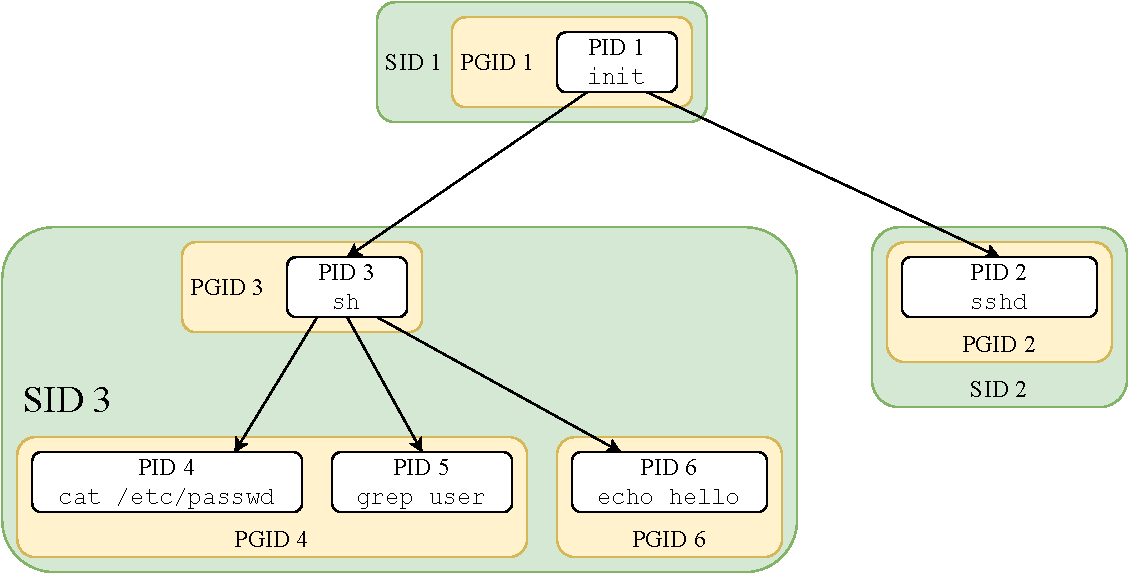
\includegraphics[width=\textwidth, keepaspectratio]{img/proc-hierarchy}
  \caption{A typical process hierarchy.}
  \label{fig:proc-hierarchy}
\end{figure}

\subsubsection{Orphaned process groups}

As we have just explained, processes belonging to the same shell job are put
inside the same process group. The shell is responsible for managing jobs, which
means keeping track of changes in their state (a job can become stopped when the
user inputs a special character), as well as manipulating them according to the
user's commands. However, when a shell exits, perhaps due to a bug, there might
no longer be a process managing these jobs. Specifically, there might no longer
be a process that can continue stopped jobs. Those jobs are doomed to being
stopped forever!

This is where the concept of \textit{orphaned process groups} comes into play. A
process group is orphaned when none of the processes in the group have a parent
that is in the same session, but in a different process group.

Consider the example of a shell: all jobs are in a different process group, but
in the same session as the shell. Therefore, as long the shell is alive, the
process groups of the jobs are not orphaned. However, when the shell process
terminates, all children of the shell are \textit{reparented}, i.e. some other
process becomes their parent, usually the \textit{init} process with PID 1. The
new parent is usually in a different session, so after reparenting the process
groups of the jobs are orphaned.

To solve the problem of jobs being stopped forever, when a process group becomes
orphaned, if the process group contains at least one stopped process, then every
process in the group is sent a \Verb{SIGHUP} signal followed by a \Verb{SIGCONT}
signal followed by \Verb{SIGHUP}. The \Verb{SIGCONT} signal will resume stopped
processes, and the \Verb{SIGHUP} signal notifies the processes that they are now
orphaned (it will also most likely kill the processes, as that is the signal's
default action).

Furthermore, processes in orphaned process groups cannot be stopped by
\textit{terminal stop signals}, i.e. \Verb{SIGTSTP}, \Verb{SIGTTOU} and
\Verb{SIGTTIN}. These signal are explained in section \ref{job-control-signals}.

\subsection{Process groups in the Mimiker kernel}

We will now describe the implementation of process groups in the Mimiker
kernel. First, we lay out the data structures used. After that, we will go over
how processes enter and exit process groups.

\subsubsection{Data structures}

\subsubsection*{\Verb{pgrp_t}}

The \Verb{pgrp_t} structure represents a single process group.

\begin{listing}[H]
\begin{minted}{c}
typedef struct pgrp {
  mtx_t pg_lock;
  TAILQ_ENTRY(pgrp) pg_hash;
  TAILQ_HEAD(, proc) pg_members;
  session_t *pg_session;
  int pg_jobc;
  pgid_t pg_id;
} pgrp_t;
\end{minted}
\caption{\texttt{include/sys/proc.h}: definition of \Verb{pgrp_t}.}
\label{lst:pgrp}
\end{listing}

The \Verb{pg_lock} mutex synchronizes concurrent accesses to the list of
members. The \Verb{pg_hash} field is a list entry used to link the structure
into the global hashtable used to lookup process groups by PGID. 

All processes that are members of the process group are on the \Verb{pg_members}
list. The list allows easy access, e.g. when a signal needs to be sent to all
members of the group.

\Verb{pg_session} is a pointer to the \Verb{session_t} structure representing
the session that this process group is a part of. Every process group is a part
of some session.

The \Verb{pg_jobc} field is a counter that tracks how many processes
\textit{qualify the group for job control}. We say that a process qualifies the
group for job control if and only if its parent is in a different process group
and in the same session. This way, when \Verb{pg_jobc} drops to zero, we know
that the process group has become orphaned.

The \Verb{pg_id} field is simply the numeric ID of the process group.

\subsubsection*{\Verb{proc_t::p_pgrp}}

The \Verb{p_pgrp} field of the process descriptor structure is a pointer to the
group that the process is a member of.

\subsubsection{Changing process groups}

Listing \ref{lst:pgrp-enter} shows kernel code implementing the POSIX
\Verb{setpgid()} function. \Verb{p} is the process that is performing the system
call, \Verb{target} is the PID of the process whose process group is to be
changed, and \Verb{pgid} is the PGID of the process group to which the target
process is to be moved.

\begin{listing}[H]
\begin{minted}{c}
int pgrp_enter(proc_t *p, pid_t target, pgid_t pgid) {
@\llabel{f1}@  SCOPED_MTX_LOCK(all_proc_mtx);
  proc_t *targetp = proc_find_raw(target);

@\llabel{f2}@  if (targetp == NULL || !proc_is_alive(targetp) ||
      (targetp != p && targetp->p_parent != p))
    return ESRCH;
@\llabel{f3}@  if (targetp == targetp->p_pgrp->pg_session->s_leader)
    return EPERM;
@\llabel{f4}@  if (targetp->p_pgrp->pg_session != p->p_pgrp->pg_session)
    return EPERM;

  pgrp_t *pg = pgrp_lookup(pgid);

  /* Create new group if one does not exist. */
@\llabel{f5}@  if (pg == NULL) {
    /* New pgrp can only be created with PGID = PID of target process. */
    if (pgid != target)
      return EPERM;
    pg = pgrp_create(pgid);
    pg->pg_session = p->p_pgrp->pg_session;
    session_hold(pg->pg_session);
@\llabel{f6}@  } else if (pg->pg_session != p->p_pgrp->pg_session) {
    /* Target process group must be in the same session
     * as the calling process. */
    return EPERM;
  }

@\llabel{f7}@  return _pgrp_enter(targetp, pg);
}
\end{minted}
\caption{\Verb{sys/kern/proc.c}: definition of \Verb{pgrp_enter()}.}
\label{lst:pgrp-enter}
\end{listing}

First, we \ref{f1} acquire the \Verb{all_proc_mtx}, which synchronizes accesses
to process-tree structures, such as process groups and sessions. Next, lines
\ref{f2}, \ref{f3} and \ref{f4} respectively perform the following checks:
\begin{itemize}
\item The target process must exist, be alive (i.e. executing normally or
  stopped), and it must either be a child of the calling process, or be the
  calling process itself;
\item The target process must not be a session leader;
\item The target process must be in the same session as the calling process.
\end{itemize}
We then \ref{f5} check whether the target process group exists. If it doesn't,
it is created, but only if the requested PGID matches the PID of the target
process. At \ref{f6} we perform yet another permission check. Finally, we call
\Verb{_pgrp_enter()} to perform the actual work of changing the process group of
the target process.

Now, let's see how a process group switch actually happens.
\begin{listing}[H]
\begin{minted}{c}
static int _pgrp_enter(proc_t *p, pgrp_t *target) {
  pgrp_t *old_pgrp = p->p_pgrp;

@\llabel{g1}@  if (old_pgrp == target)
    return 0;

@\llabel{g2}@  pgrp_jobc_enter(p, target);
  pgrp_jobc_leave(p, old_pgrp);

@\llabel{g3}@  WITH_MTX_LOCK(&old_pgrp->pg_lock) {
    WITH_MTX_LOCK(&target->pg_lock) {
      WITH_PROC_LOCK(p) {
@\llabel{g4}@        TAILQ_REMOVE(&old_pgrp->pg_members, p, p_pglist);
        TAILQ_INSERT_HEAD(&target->pg_members, p, p_pglist);
        p->p_pgrp = target;
      }
    }
  }

@\llabel{g5}@  if (TAILQ_EMPTY(&old_pgrp->pg_members))
    pgrp_remove(old_pgrp);

  return 0;
}
\end{minted}
\caption{\Verb{sys/kern/proc.c}: definition of \Verb{_pgrp_enter()}.}
\label{lst:-pgrp-enter}
\end{listing}

We first \ref{g1} check whether we need to change groups at all. If we do, we
\ref{g2} adjust the \Verb{pg_jobc} counters of the old group, target group, as
well as the process groups of all children of the process. We will examine these
functions in a minute.

The process group switch must appear atomic. For this reason, it is necessary to
hold \Verb{all_proc_mtx}, both the old group and target group's lock, and the
process lock of the target process. We acquire the necessary locks at \ref{g3}.
\Verb{all_proc_mtx} is not acquired, since it is already held by the caller of
\Verb{_pgrp_enter()}.

When acquiring two locks of the same type (in this case process group locks),
one has to be very careful not to cause a deadlock. The usual way to ensure
safety from deadlocks is to establish an order on the locks, and whenever
multiple locks need to be acquired, make sure all required locks are acquired
according to that order. However, in this case deadlock can be avoided without
specifying an order on process group locks, by enforcing the following rule:
\begin{quote}
  In order to acquire multiple process group locks, a thread must already hold
  the \Verb{all_proc_mtx} lock.
\end{quote}
With this rule in force, it is impossible for two threads to concurrently
attempt to acquire multiple process group locks, since \Verb{all_proc_mtx} will
act as a serializer between them. The rule is a natural fit in this particular
situation for two reasons:
\begin{itemize}
  \item \Verb{_pgrp_enter()} is the only place in the whole kernel where there
    is a need to acquire multiple process group locks;
  \item The \Verb{all_proc_mtx} lock is already held everywhere
    \Verb{_pgrp_enter()} is called. Therefore, virtually no code changes had to
    be made in order to accomodate this rule.
\end{itemize}

At \ref{g4}, we are finally ready to make the switch. We remove the process from
the old group's list of members, add it to the target group's list, and change
the \Verb{p_pgrp} pointer.

At the end, we \ref{g5} check whether the process was the last remaining process
in the old group. If so, the process group is removed.

\subsubsection{Orphaned process groups}

The \Verb{pg_jobc} counters need to be adjusted whenever a process leaves or
enters a process group. However, it is not sufficient to adjust only the counter
of the process group being entered or left. When a process leaves a process
group, the children of the process may no longer qualify their process group for
job control.

Figure \ref{fig:orphan} illustrates a scenario in which a call to
\Verb{setpgid()} causes the process group of a child of the calling process to
become orphaned. For this reason, it is necessary to check whether the children
still qualify their process groups for job control whenever leaving or entering
a process group.

\begin{figure}[h]
  \centering
  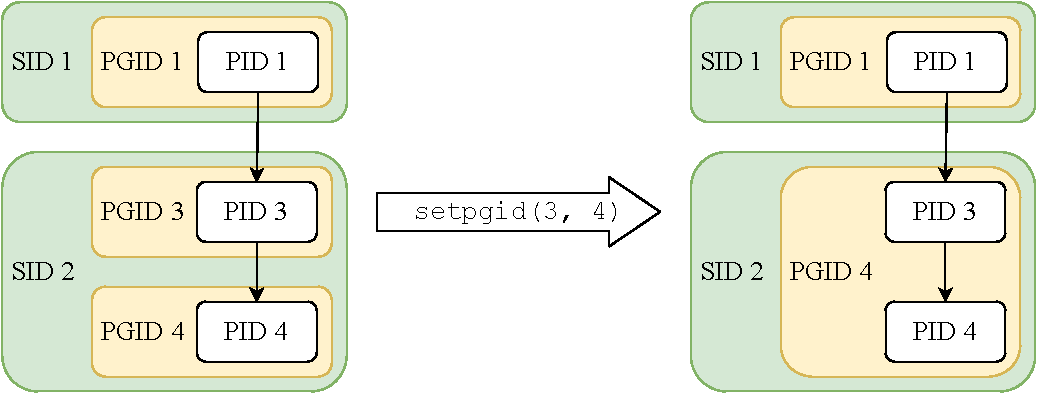
\includegraphics[width=\textwidth, keepaspectratio]{img/orphan}
  \caption{A parent's change of process group causes a child's process group to
    become orphaned.}
  \label{fig:orphan}
\end{figure}

The accounting associated with \Verb{pg_jobc} is split into two functions:\\
\Verb{pgrp_jobc_enter()} and \Verb{pgrp_jobc_leave()}.

\begin{listing}[H]
\begin{minted}{c}
static void pgrp_jobc_enter(proc_t *p, pgrp_t *pg) {
  assert(mtx_owned(all_proc_mtx));

@\llabel{h1}@  if (same_session_p(p->p_parent->p_pgrp, pg))
    pg->pg_jobc++;

  proc_t *child;
@\llabel{h2}@  TAILQ_FOREACH (child, CHILDREN(p), p_child)
    if (same_session_p(child->p_pgrp, pg))
      child->p_pgrp->pg_jobc++;
}
\end{minted}
\caption{\Verb{sys/kern/proc.c}: definition of \Verb{pgrp_jobc_enter()}.}
\label{lst:-pgrp-enter}
\end{listing}

\Verb{p} is the process entering the process group \Verb{pg}.
The \Verb{same_session_p()} function returns \Verb{true} if and only if the two
groups are different, but in the same session.

At \ref{h1}, we check whether \Verb{p} will qualify the process group \Verb{pg}
for job control after entering it. If so, the \Verb{pg_jobc} counter is
incremented.

Next, at \ref{h2} we do the same for the children of \Verb{p}: we check whether
they will qualify their process groups after \Verb{p} enters \Verb{pg}. If so,
the group's \Verb{pg_jobc} is incremented.

The \Verb{pgrp_jobc_leave()} function has a very similar structure, except now
we call \Verb{pgrp_maybe_orphan()} instead of incrementing \Verb{pg_jobc}. The
\Verb{pgrp_maybe_orphan()} function decrements the process group's
\Verb{pg_jobc}, and if it reaches zero, sends the appropriate signals.

\begin{listing}[H]
\begin{minted}{c}
static void pgrp_jobc_leave(proc_t *p, pgrp_t *pg) {
  assert(mtx_owned(all_proc_mtx));

  if (same_session_p(p->p_parent->p_pgrp, pg))
    pgrp_maybe_orphan(pg);

  proc_t *child;
  TAILQ_FOREACH (child, CHILDREN(p), p_child)
    if (same_session_p(child->p_pgrp, pg))
      pgrp_maybe_orphan(child->p_pgrp);
}
\end{minted}
\caption{\Verb{sys/kern/proc.c}: definition of \Verb{pgrp_jobc_leave()}.}
\label{lst:-pgrp-enter}
\end{listing}

\subsection{Sessions in the Mimiker kernel}

We will now examine the implementation of sessions in the Mimiker kernel. After
looking at the session data structure, we will see how new sessions are created.

\subsubsection{Data structures}

The \Verb{session_t} data structure represents a single session. Listing
\ref{lst:sess} presents its complete definition.

\begin{listing}[H]
\begin{minted}{c}
typedef struct session {
  TAILQ_ENTRY(session) s_hash;
  proc_t *s_leader;
  int s_count;
  sid_t s_sid;
  tty_t *s_tty;
  char s_login[LOGIN_NAME_MAX];
} session_t;
\end{minted}
\caption{\Verb{include/sys/proc.h}: definition of \Verb{session_t}.}
\label{lst:sess}
\end{listing}

The \Verb{s_hash} field is used to link the structure into the hashtable used to
look up session strucutures by their session ID (SID).

The \Verb{s_leader} field points to the process that is the session leader, i.e.
the process that created the session by calling the \Verb{setsid()} function.
Once the session leader terminates, the \Verb{s_leader} field of the session is
set to \Verb{NULL}.

The \Verb{s_count} field counts the number of process groups belonging to the
session. Whenever a new process group joins the session, the
\Verb{session_hold()} function increments the \Verb{s_count} field (see listing
\ref{lst:pgrp-enter} for an example of its usage). When a process group is
removed, the \Verb{pgrp_remove()} function, which can be seen used in listing
\ref{lst:-pgrp-enter} decrements the session's \Verb{s_count} field. Once the
value of the field reaches zero, the session is removed from the kernel and the
memory occupied by the structure is reclaimed.

The \Verb{s_sid} field holds the numeric ID of the session. It is equal to the
PID of the process that created the session.

The \Verb{s_tty} field is a pointer to the session's controlling terminal. For
interactive sessions (i.e. sessions created by a user logging into the system
and launching a shell), the controlling terminal is the device that provides
input to the shell and spawned jobs, and receives their output. Not every
session has a controlling terminal: daemon processes are usually placed in
sessions without a controlling terminal. If a session has no controlling
terminal, the value of its \Verb{s_tty} field is set to \Verb{NULL}.

\subsubsection{Creating a session}

User processes can create new sessions using the \Verb{setsid()} function from
the C library. That function directly calls the \Verb{setsid()} system call,
which is implemented by the \Verb{sys_setsid()} function in the kernel. That
function, in turn, calls \Verb{session_enter()} to do the work. Listing
\ref{lst:session-enter} presents the source code of \Verb{session_enter()}.

\begin{listing}[H]
\begin{minted}{c}
int session_enter(proc_t *p) {
@\llabel{i1}@  SCOPED_MTX_LOCK(&all_proc_mtx);

  pgid_t pgid = p->p_pid;
  pgrp_t *pg = pgrp_lookup(pgid);

@\llabel{i2}@  if (pg)
    return EPERM;

@\llabel{i3}@  pg = pgrp_create(pgid);
@\llabel{i4}@  pg->pg_session = session_create(p);

@\llabel{i5}@  return _pgrp_enter(p, pg);
}
\end{minted}
\caption{\Verb{sys/kern/proc.c}: definition of \Verb{session_enter()}.}
\label{lst:session-enter}
\end{listing}

First, we \ref{i1} acquire the \Verb{all_proc_mtx} lock, which is required to perform
things such as process group lookups and creating new sessions and process
groups.

At \ref{i2}, we ensure that there doesn't already exist a process group with the
same PGID as the PID of the calling process. The process group that is created as
a result of creating a new session has a PGID equal to the PID of the calling
process, and if a group with such a PGID already exists, we can't create the
group we need, since PGIDs must be unique.

Once we have ensured that we can create the group, we do so at \ref{i3}. Then,
we \ref{i4} create a new session with \Verb{p} as the session leader and link it
to the newly created group (the session created by \Verb{session_create()} has a
\Verb{s_count} of 1, so there's no need to adjust it). Finally, we \ref{i5}
change the process group of the calling process to the one we just created.

\section{Job Control Signals}

\subsection{POSIX signals}

\textit{Signals} are used to notify processes of various events. These events
can occur \textit{synchronously} or \textit{asynchronously} with respect to the
process receiving the signal. POSIX signal semantics are (intentionally) very
similar to those found in the original UNIX operating system
\cite[Section~7.2]{unix-book}.

A \textit{synchronous signal} is sent as a direct consequence of some (usually
erroneous) action being performed by the receiving process. For instance, a
process is sent a \texttt{SIGSEGV} signal upon trying to access an invalid
memory location.

An \textit{asynchronous signal} is sent independently of the actions of the
receiving process, and may be received at any time. For example, whenever a
process terminates, the system sends a \texttt{SIGCHLD} signal to its parent.

Signals can be sent by the operating system in response to certain events (e.g.
process termination), or by other processes, using the \texttt{kill()} function
\cite{kill}. A process can send a signal to itself using the \texttt{raise()}
function. As a shorthand, we shall say that a signal is sent to a process
group when it's sent to every process that is a member of the group.

The type of signal (\texttt{SIGSEGV}, \texttt{SIGCHLD}, etc.) is determined by
the \textit{signal number}. In fact, \texttt{SIGSEGV} and others are \textit{C
  preprocessor macros} that expand to unique signal numbers.

Processes can take different actions in response to signals with different
numbers. Every process has its own set of \textit{signal actions} associated
with every signal number. There are three possible actions that can be taken in
response to a signal:
\begin{enumerate}
\item Take the default action for that signal number.
  
  Every signal number has an associated default action. For instance, the
  default action of the \texttt{SIGSEGV} signal is to immediately terminate the
  receiving process.
\item Ignore the signal.
\item Invoke a \textit{signal handler routine}.

  The handler routine is run in the context of the process that receiving
  process. After the handler finishes execution, the process is resumed.
\end{enumerate}

The mapping of signal numbers to signal actions is controlled using the
\texttt{sigaction()} function \cite{sigaction}. Not every signal can have its
action modified: \texttt{SIGKILL} and \texttt{SIGSTOP} cannot have their actions
changed from the default one, which is to terminate or stop the receiving process,
respectively.

The \textit{delivery} of a signal occurs when the target (i.e. receiving)
process takes the action associated with the signal. A signal may be delivered
long after it is initially sent, or it may not be delivered at all, even if it
isn't ignored. This is because a process may \textit{block} a set of signals
from being delivered. A blocked signal cannot be delivered until it is
unblocked. Contrary to signals that are ignored, blocked signals await delivery
instead of being discarded.

The \textit{signal mask} determines the set of blocked signals for a thread. It
can be examined and modified using the \texttt{sigprocmask()} function
\cite{sigprocmask}. Unsurprisingly, the \texttt{SIGKILL} and \texttt{SIGSTOP}
signals cannot be blocked from being delivered.

\subsection{Signals used for job control}
\label{job-control-signals}

The following signals are most commonly used to control jobs on POSIX-compliant
operating systems:
\begin{itemize}
\item \texttt{SIGINT}

  Sent by the operating system in response to the special
  character \texttt{VINTR} being received on the terminal. Its purpose is to
  signal interruption by the user. A process that receives this signal is
  usually expected to terminate shortly. The default action associated with this
  signal is to terminate the receiving process.

\item \texttt{SIGQUIT}

  Similar to \texttt{SIGINT}, except it is sent in response to the
  \texttt{VQUIT} character, and the default action additionally generates a core
  dump of the receiving process.

\item \texttt{SIGTTOU}

  Sent by the operating system whenever a background job attempts to write to
  the terminal, provided the \texttt{TOSTOP} terminal flag is set (more on
  terminal flags later). The default action associated with this signal is to
  stop the receiving process.
  
\item \texttt{SIGTTIN}

  Sent by the operating system whenever a background job attempts to read from
  the terminal. Background jobs may not read from the terminal, regardless of
  the terminal settings. The default action associated with this signal is to
  stop the receiving process.

\item \texttt{SIGTSTP}

  Sent by the operating system in response to the special character
  \texttt{VSUSP} being received on the terminal. Its purpose is to stop the
  foreground job. Well-behaving processes should not ignore this signal. Many
  programs need to do some cleanup before stopping: in that case, they register
  a handler that does the necessary cleanup, after which it performs
  \texttt{raise(SIGSTOP)}. The default action associated with this signal is to
  stop the receiving process.

\item \texttt{SIGSTOP}

  This signal is not sent by the operating system. It unconditionally stops the
  receiving process. It cannot be blocked or ignored. 

\item \texttt{SIGCONT}

  This is the only signal that can resume a stopped process (apart from
  \texttt{SIGKILL}, which resumes it only to immediately terminate it). It is
  usually sent by the shell, e.g. when a background job that was stopped by a
  \texttt{SIGTTIN} signal is brought into the foreground.

\item \texttt{SIGCHLD}

  Sent by the operating system in response to the termination of a process. The
  signal is sent to the parent of the terminating process. Shells use this
  signal to update their data on currently running jobs.
\end{itemize}

\subsection{Signals in the Mimiker kernel}

In this subsection we describe the implementation of signals in the Mimiker
kernel. First, we lay out the data structures used, after which we go through
how exactly signals are sent and delivered in the kernel. Lastly, we examine how
processes are stopped in response to the delivery of a stop signal.

\subsubsection{Signal data structures}

We will now describe the various data types and structures that are critical to
the implementation of signals in the Mimiker kernel.

\subsubsection*{\Verb{sigaction_t}}


The \Verb{sigaction_t} data type describes the disposition of a signal.
\begin{listing}[H]
\begin{minted}{c}
typedef void (*sig_t)(int); /* type of signal function */

typedef struct sigaction {
  union {
    sig_t sa_handler;
    void (*sa_sigaction)(int, siginfo_t *, void *);
  };
  sigset_t sa_mask;
  int sa_flags;
} sigaction_t;
\end{minted}
\caption{\texttt{include/sys/signal.h}: definition of \Verb{sigaction_t}.}
\end{listing}

The \Verb{sa_handler} and \Verb{sa_sigaction} fields are
simply pointers to a signal handler function. Processes can register either a
handler of type \Verb{sig_t}, which takes only the signal number as an
argument, or a handler that takes two additional arguments:
\begin{itemize}
\item A pointer to a structure of type \Verb{siginfo_t}, which contains
  more information about the signal (e.g. in the case of
  \Verb{SIGCHLD}, the PID of the child process);

\item A pointer that can be cast to a pointer to a structure of type
  \Verb{ucontext_t}, which holds the processor context of the thread
  that received the signal at the time of the signal's delivery.
\end{itemize}
The \Verb{sa_handler} field can also have the special value
\Verb{SIG_DFL} or \Verb{SIG_IGN}, which respectively mean
that the signal has the default disposition or is ignored.

The \Verb{sa_mask} field is the set of signals that are blocked
during the execution of the handler function. After the handler finishes, the
signal mask is restored to its previous state.
 
The \Verb{sa_flags} field is a set of flags that modify the behaviour
of the signal in various ways. At the time of writing, the only flag supported
in the Mimiker kernel is \Verb{SA_RESTART}, which causes system calls
that are interrupted by a signal handler to be automatically restarted,
transparently to the process that issued the system call.

\subsubsection*{\Verb{proc_t::p_sigactions}}

The \Verb{p_sigactions} field of the \Verb{proc_t} (i.e.
process descriptor) structure is an array of structures of type
\Verb{sigaction_t}. For each signal number \Verb{signo}, the
disposition of that signal for the process is stored in
\Verb{p_sigactions[signo]}.

\subsubsection*{\Verb{thread_t::td_sigmask}}

As opposed to the signal disposition, which is shared by all the threads of a
process, every thread has its own set of blocked signals. This set is stored in
the \Verb{td_sigmask} field of the \Verb{thread_t} structure,
which describes a single thread of execution. The field is just a bit vector,
with each bit corresponding to a signal number. If a bit is set, signals with
the corresponding number are blocked from being delivered.

\subsubsection*{\Verb{thread_t::td_sigpend}}

The \Verb{td_sigpend} field of the \Verb{thread_t} structure
represents pending signals, i.e. signals that have been sent to the thread and
are waiting to be delivered. It is a structure of type
\Verb{sigpend_t}, which consists of a bit vector of pending signal
numbers, as well as a list of \Verb{ksiginfo_t} structures which carry
additional information about signals.

\subsubsection{Sending a signal}

We will now walk through the code that does the actual work of sending a signal
to a process. Sending signals in the Mimiker kernel is accomplished using the
\Verb{sig_kill()} function. Listing \ref{lst:sig-kill} contains slightly
simplified code of the function.

\begin{listing}[H]
\begin{minted}{c}
void sig_kill(proc_t *p, ksiginfo_t *ksi) {
@\llabel{a1}@  assert(mtx_owned(&p->p_lock));

  signo_t sig = ksi->ksi_signo;
  thread_t *td = p->p_thread;
  bool ignored = sig_ignored(p->p_sigactions, sig);

@\llabel{a2}@ if ((ignored && !sigprop_cont(sig)) || sig_ignore_ttystop(p, sig))
    return;

  /* If sending a stop or continue signal,
   * remove pending signals with the opposite effect. */
@\llabel{a3}@  if (defact_stop(sig)) {
    sigpend_get(&td->td_sigpend, SIGCONT, NULL);
  } else if (sigprop_cont(sig)) {
    sigpend_delete_set(&td->td_sigpend, &stopmask);
@\llabel{a4}@    if (p->p_state == PS_STOPPED)
      proc_continue(p);
    if (ignored)
      return;
  }

@\llabel{a5}@  sigpend_put(&td->td_sigpend, ksiginfo_copy(ksi));

@\llabel{a6}@  if (__sigismember(&td->td_sigmask, sig))
    return;

  WITH_SPIN_LOCK (td->td_lock) {
@\llabel{a7}@    td->td_flags |= TDF_NEEDSIGCHK;
    if (td_is_interruptible(td)) {
      spin_unlock(td->td_lock);
      sleepq_abort(td); /* Locks & unlocks td_lock */
      spin_lock(td->td_lock);
    }
  }
}
\end{minted}
\caption{\Verb{sys/kern/signal.c}: definition of \Verb{sig_kill()}.}
\label{lst:sig-kill}
\end{listing}

The function accepts two parameters. The first is a pointer to a \Verb{proc_t}
structure, which represents the process that the signal will be sent to. The
second is a pointer to a \Verb{ksiginfo_t} structure, which describes the signal
to be sent. Most importantly, it contains the signal number.

The assertion at \ref{a1} ensures that the function's caller has acquired the
necessary lock. Processes' and threads' signal data structures are globally
shared (i.e. many threads of execution can access them), so access to them must
be synchronized using locks.

We then \ref{a2} quickly filter out ignored signals, with an exception for
signals that can continue stopped processes, as some processing needs to be done
even if they are ignored. Furthermore, terminal stop signals (\Verb{SIGTSTP},
\Verb{SIGTTOU} and \Verb{SIGTTIN}) cannot stop a process which is in an orphaned
process group: this case is detected by the \Verb{sig_ignore_ttystop()} function.

In \ref{a3}, we check whether the signal being sent is a stop or continue
signal. If it is, we remove all signals that are already pending which have the
opposite effect. Additionally, for continue signals \ref{a4} we check whether
the target process is stopped. If it is, we wake it up and notify its parent.

Once control reaches \ref{a5}, we are certain that the signal isn't ignored, so
it should be queued for delivery to the target process. The \Verb{sigpend_put}
function inserts the signal into the set of pending signals for the target
process's thread.

The final step is notifying the thread that it needs to process its pending
signals. This step is skipped if \ref{a6} the signal is blocked from being
delivered. The \Verb{TDF_NEEDSIGCHK} flag lets the thread know that it should
check for pending signals at the nearest opportunity. If the thread is
\textit{sleeping interruptibly} (e.g. blocked inside a \Verb{read()} call on a
terminal device, awaiting user input), it is awakened so that it can receive the
signal.


\subsubsection{Signal delivery}

After a signal is sent, it remains in the pending set, waiting to be delivered.
Signals are delivered to a process whenever control transfers from the kernel
to that process, i.e. on transitions from the kernel to userspace. For instance,
pending signals are delivered before returning from a system call. 

Signal delivery can be divided into two steps: checking for a pending signal,
and \textit{posting} a signal found to be pending. Posting a signal means
setting up the execution context of the process, so that the signal handler is
the first thing that is executed after returning control to the process.

Signals with special effects (i.e. stopping or killing a process) are not
posted, but are instead handled as part of checking for a pending signal. This
is an implementation choice that simplifies handling of certain edge cases.

Pending signals are not checked at all if the current thread does not have the
\Verb{TDF_NEEDSIGCHK} flag set. This flag is set in \Verb{sig_kill()}, see
listing \ref{lst:sig-kill}. This saves us from unnecessarily checking for
pending signals every time we return to userspace.

We will not describe how signals are posted, as most of the details are
architecture-specific, and we are primarily concerned with job control signals,
which are not posted at all (unless they have registered handlers, in which case
they don't behave like job control signals). Instead, we will focus on the
\Verb{sig_check()} function, which checks for pending signals and handles job
control signals. Listing \ref{lst:sig-check} contains the source code of the
function.

\begin{listing}[H]
\begin{minted}{c}
int sig_check(thread_t *td, ksiginfo_t *out) {
  proc_t *p = td->td_proc;
  signo_t sig;

@\llabel{b0}@  assert(mtx_owned(&p->p_lock));

@\llabel{b1}@  while ((sig = sig_pending(td))) {
@\llabel{b2}@    sigpend_get(&td->td_sigpend, sig, out);

@\llabel{b3}@    if (sig_should_stop(p->p_sigactions, sig)) {
      if (!sig_ignore_ttystop(p, sig))
        proc_stop(sig);
      continue;
    }

@\llabel{b4}@    if (sig_should_kill(p->p_sigactions, sig))
      sig_exit(td, sig);

@\llabel{b5}@    return sig;
  }

  WITH_SPIN_LOCK (td->td_lock)
@\llabel{b6}@    td->td_flags &= ~TDF_NEEDSIGCHK;
@\llabel{b7}@  return 0;
}
\end{minted}
\caption{\Verb{sys/kern/signal.c}: definition of \Verb{sig_check()}.}
\label{lst:sig-check}
\end{listing}

This function manipulates signal state, which is protected by the process's
lock, hence the assertion at \ref{b0}.

The function first \ref{b1} extracts a pending signal that is not currently
blocked using the \Verb{sig_pending()} function. It returns just a signal
number, so in the next step \ref{b2} we remove the signal from the set of
pending signals.

We then check \ref{b3} if the signal should stop the receiving process. Notice
that after stopping the process with \Verb{proc_stop()}, control goes back to
\ref{b1}.

Next, we \ref{b4} handle signals that should kill the process. The
\Verb{sig_exit()} function never returns.

If the pending signal is neither a stop nor a kill signal, \ref{b5} the signal
number is returned. Additional information about the signal is passed to the
caller via the \Verb{out} output parameter. The signal is then passed to
\Verb{sig_post()} to arrange for the handler to be called.

If no signal needs to be posted, the function \ref{b6} clears the thread's
\Verb{TDF_NEEDSIGCHK} flag, since there is no need to check for pending signals
anymore. A return value of 0 \ref{b7} indicates to the caller that no signal
needs to be posted.

\subsubsection{Stopping and continuing processes}

One of the job control features that were implemented from scratch as part of
the implementation effort described in this thesis is support for stopping and
continuing processes by means of the \Verb{SIGSTOP} and \Verb{SIGCONT} signals.

A process is always in one of several states, denoted by the value of the
\Verb{p_state} field in the process descriptor. When a process is executing
normally, its state is \Verb{PS_NORMAL}. When a process is stopped, its state is
\Verb{PS_STOPPED}. All the threads of a stopped process are also stopped and
unable to run until the process is continued.

The \Verb{proc_stop()} function stops the current process in response to a stop
signal. Its source code is listed in listing \ref{lst:proc-stop}.

\begin{listing}[H]
\begin{minted}{c}
void proc_stop(signo_t sig) {
  thread_t *td = thread_self();
  proc_t *p = td->td_proc;

@\llabel{c1}@ assert(mtx_owned(&p->p_lock));
  assert(p->p_state == PS_NORMAL);

@\llabel{c2}@  p->p_state = PS_STOPPED;
@\llabel{c3}@  p->p_stopsig = sig;
  p->p_flags |= PF_STATE_CHANGED;
  WITH_PROC_LOCK(p->p_parent) {
@\llabel{c4}@    proc_wakeup_parent(p->p_parent);
    sig_child(p, CLD_STOPPED);
  }
@\llabel{c5}@  WITH_SPIN_LOCK (td->td_lock) { td->td_flags |= TDF_STOPPING; }
  proc_unlock(p);
  /* We're holding no locks here, so our process can be continued before we
   * actually stop the thread. This is why we need the TDF_STOPPING flag. */
  spin_lock(td->td_lock);
@\llabel{c6}@  if (td->td_flags & TDF_STOPPING) {
    td->td_flags &= ~TDF_STOPPING;
    td->td_state = TDS_STOPPED;
@\llabel{c7}@    sched_switch(); /* Releases td_lock. */
  } else {
    spin_unlock(td->td_lock);
  }
  proc_lock(p);
  return;
}
\end{minted}
\caption{\Verb{sys/kern/proc.c}: definition of \Verb{proc_stop()}.}
\label{lst:proc-stop}
\end{listing}

This function manipulates process state, hence the assertion at \ref{c1}. The
next assertion simply makes sure that the process is in the expected state.
Next, at \ref{c2} the process state is set to \Verb{PS_STOPPED}.

At \ref{c3}, we set up information that is used by the \Verb{wait4()} system
call. It is used by a process to wait for one of its children to change state.
As the reader might have already guessed, stopping counts as a state change. The
call to \Verb{proc_wakeup_parent()} at \ref{c4} notifies the parent process of
the status change. In the next line, a \Verb{SIGCHLD} signal is sent to the
parent.

The rest of the function attempts to stop the process's thread. This task is
fairly simple, due to the fact that all processes in the Mimiker kernel are
single-threaded. Still, it is not as simple as one might like, due to some
technicalities around locking.

Specifically, we are not allowed to hold the thread's spinlock
(\Verb{td->td_lock}) while releasing a mutex. Furthermore, we must release the
process's lock before stopping the thread in \Verb{sched_switch()}, and the
thread's spinlock must be held when calling \Verb{sched_switch()}. These
constraints require us to briefly hold no locks at all. During this window of
time, another process might continue the process we are trying to stop, in which
case we should not stop the thread.

The solution is to add the \Verb{TDF_STOPPING} thread flag, which signals that
the thread is about to stop, but hasn't stopped yet. It is set \ref{c5} while
still holding the process's lock. If the process is continued before the thread
is stopped, the \Verb{TDF_STOPPING} flag is cleared. The stopping thread
examines \ref{c6} the flag before changing its state. Thanks to this, the thread
will stop only if the process is still stopped.

After setting the thread state to \Verb{TDS_STOPPED}, the call \ref{c7} to
\Verb{sched_switch()} hands over control to the scheduler, which will select
another thread to run. The stopped thread will not be selected by the scheduler
to run until it is continued.

Let us now see how stopped processes are woken up. Continuing a process is
simpler than stopping one, as can be seen by looking at listing \ref{lst:proc-continue}. 

\begin{listing}[H]
\begin{minted}{c}
void proc_continue(proc_t *p) {
  thread_t *td = p->p_thread;

@\llabel{d1}@  assert(mtx_owned(&p->p_lock));
  assert(p->p_state == PS_STOPPED);

@\llabel{d2}@  p->p_state = PS_NORMAL;
@\llabel{d3}@  p->p_flags |= PF_STATE_CHANGED;
  WITH_PROC_LOCK(p->p_parent) {
    proc_wakeup_parent(p->p_parent);
  }
@\llabel{d4}@  WITH_SPIN_LOCK (td->td_lock) { thread_continue(td); }
}
\end{minted}
\caption{\Verb{sys/kern/proc.c}: definition of \Verb{proc_continue()}.}
\label{lst:proc-continue}
\end{listing}

The assertion at \ref{d1} should come as no surprise at this point, as we are
modifying the process's state. The next assertion ensures that we only attempt
to continue processes that are actually stopped.

We then \ref{d2} restore the process's \Verb{p_state} to \Verb{PS_NORMAL}. Next,
we \ref{d3} notify the parent of the state change. Note that, in contrast to
\Verb{proc_stop()}, we don't send a \Verb{SIGCHLD} signal to the parent process.
This is in line with the POSIX specification.

Lastly, we \ref{d4} wake up the thread of the process we are continuing. The
\Verb{thread_continue()} function is very simple, and is presented in listing
\ref{lst:thread-continue}.

\begin{listing}[H]
\begin{minted}{c}
void thread_continue(thread_t *td) {
@\llabel{e1}@  if (td->td_flags & TDF_STOPPING) {
    td->td_flags &= ~TDF_STOPPING;
  } else {
@\llabel{e2}@    assert(td_is_stopped(td));
@\llabel{e3}@    sched_wakeup(td, 0);
  }
}
\end{minted}
\caption{\Verb{sys/kern/thread.c}: definition of \Verb{thread_continue()}.}
\label{lst:thread-continue}
\end{listing}

An important thing to notice is that even if a process's state indicates that it
is stopped (i.e. \Verb{p_state == PS_STOPPED}), its thread is not guaranteed to
also be stopped (i.e. \Verb{td_state == TDS_STOPPED}). The call to
\Verb{proc_continue()} can occur at the time in \Verb{proc_stop()} where we are
not holding any locks.

For this reason, we first \ref{e1} check the \Verb{TDF_STOPPING} flag. If it is
set, the thread has not stopped yet, and all we need to do is clear the flag.
If the flag is not set, then we know that the thread is stopped, hence the
assertion at \ref{e2}. We then \ref{e3} call \Verb{sched_wakeup()} to make the
thread runnable again.

The primary way of controlling a computer over a terminal connection
 is using a
\textit{shell}. A shell is a program that executes commands typed by the user.
The purpose of most commands is to run a specified program with a given set of
arguments. For example, the command \texttt{ls -l} instructs the shell to find a
program named \texttt{ls} and run it with a single argument \texttt{-l}.
The executed program will then run to completion. It may accept further input
from the user and write output. The shell waits for the program to finish, after
which it is ready to accept more commands from the user.

This example presented a very simple use case.
The user may want to execute \textit{jobs} that consist of a pipeline of
programs, with programs in the middle of the pipeline accepting input from the
previous one and feeding output to the next one. Such jobs may run for a long
time, so the user should be able to run any job in the background, without
making the shell wait for it to finish.

\textit{Job control} is a general feature of the system that allows the user to
control running jobs. A job may be suspended and resumed, terminated, a
background job may be brought into the foreground and vice versa. Job control
usually requires support from the operating system, and it's up to the shell to
group related programs into jobs.

\chapter{The Terminal Subsystem}

TODO Zrobić coś z tym i POSIX Job Control
\section{What is POSIX?}

POSIX~\cite{posix} is a set of standards specifying an operating system
interface. Its primary goal is to make it easy to write portable libraries and
applications that work across different operating systems, although they usually
need to be compiled for each operating system separately.

Among other things, it defines an Application Programming Interface (API) for
programs written in the C programming language that allows them to interact with
the system and use its services. Every POSIX-compliant operating system must
provide an implementation of this API.

The Mimiker operating system implements the POSIX API, but the implementation is
far from complete. This allows us to use existing programs using the POSIX API
like shells, command line utilities and text editors.

\section{POSIX Job Control}

\subsection{Jobs}
A job consists of one or more processes. The processes are usually connected in
a pipeline, with each one accepting input from the previous one in the chain,
and feeding output to the next one.

Jobs are purely a shell concept: they are implemented entirely in the shell,
and the operating system has no knowledge of them. However, there is a close
correspondence between shell jobs and process groups, which are implemented by
the operating system. The shell puts different jobs in different process groups.

\section{POSIX Terminals}
On the surface, a terminal device is no different than a standard characters
device: a process can open it using \texttt{open()} and then perform input and
output using \texttt{read()} and \texttt{write()} respectively.
The terminal interface specified by POSIX is much richer than that. Terminal
devices play a significant role in job control, and therefore are connected to
the concepts of process groups and sessions.

\subsection{Controlling terminals}
A terminal device may be the controlling terminal of a session. A session may
have at most one controlling terminal, and a terminal device may be the controlling
terminal of at most one session. A process can always access its controlling
terminal (if it has one) by opening the \texttt{/dev/tty} device file.

When a session is created, it has no controlling terminal. The session leader is
responsible for setting and changing the controlling terminal device, although
the way in which this is done is not specified in the standard.

When the leader of a session terminates, the controlling terminal (if any) is
dissociated from the session. Any processes left in the session may have their
access to the controlling terminal revoked. If a controlling terminal device
disappears from the system, the leader of the associated session is sent a
\texttt{SIGHUP} signal.

\subsection{Foreground process groups}
Access to the controlling terminal by processes can be controlled using
foreground and background process groups.

At any time, a process group can be designated as the foreground process group
of its session's controlling terminal. All other process groups in the session
are background process groups. The foreground process group of a terminal can be
set using the \texttt{tcsetpgrp()}\cite{tcsetpgrp} function. Any process can set
the foreground process group of its controlling terminal, although some
restrictions apply to processes from background process groups. A controlling
terminal does not need to have a foreground process group at all times.

Processes in the foreground process group are allowed to \texttt{read()} and
\texttt{write()} to their controlling terminal. When a process in a background
process group attempts to \texttt{read()} or \texttt{write()} to its controlling
terminal, every process in its process group is sent a \texttt{SIGTTIN} or
\texttt{SIGTTOU} signal respectively. The default effect of both signals is to
stop the target process. In the case of \texttt{write()}, the signal is sent
only if the \texttt{TOSTOP} terminal flag is set. If it is not set, background
processes can write to their controlling terminal without restrictions. The
exact semantics are a bit more nuanced, see \cite{terminal-access}.

When a shell is accepting input from the user, its process is necessarily in the
foreground process group. When the shell starts a job, the job is usually put in
the foreground, so that the user can interact with it. The shell waits for the
foreground job to complete, and then makes its own process group the foreground
process group, so that it can accept the next command.

The user may make the job run in the background by appending \texttt{\&} to the
command. In that case, the shell remains in the foreground process group and
does not wait for the job to complete. As explained earlier, a background job
will be stopped if it tries to accept input from the user.

A background job can be put in the foreground using the \texttt{fg} command. The
command simply sets the controlling terminal's foreground process group to the
process group of the target job, continues the target job if it was stopped, and
waits for the foreground job's termination.

\subsection{Terminal modes and flags}

Command line applications can be roughly divided into two groups, depending on
how they process user input:
\begin{itemize}
  \item{One line at a time (\textit{line-oriented});}
  \item{One character at a time (\textit{character-oriented}).}
\end{itemize}

A shell belongs to the first group. It accepts a whole command at a time. Most
notably, the user may edit the line before submitting it to the program by
pressing the return key (labelled ``enter'' on most keyboards).

A text editor belongs to the second group. Each key performs an action within
the editor, such as moving the cursor or inserting text at the position of the
cursor.

In serious applications, line-oriented input is usually accomplished using a
library such as GNU Readline \cite{readline}. However, POSIX mandates that basic
line-editing functionality is provided by the operating system itself.
Applications may choose whether they want to use this functionality by choosing
the \textit{terminal mode}.

Two terminal modes are distinguished: \textit{canonical} and
\textit{non-canonical} (often called \textit{raw}). Canonical mode provides
basic line editing:
\begin{itemize}
  \item{Characters typed by the user are ``echoed'' to the terminal;}
  \item{Characters may be erased from the line.}
\end{itemize}
It also causes certain actions to be taken in response to special
\textit{control characters} being received.

Character echoing allows the user to see the contents of the line they are
typing. This is necessary for the user to be able to spot mistakes in their
input. It is sometimes useful to turn off character echoing, e.g. when the user
is typing their password.

Characters can be erased from the line by sending certain control characters.
For instance, the \texttt{VERASE} character erases the character at the end of
the line, and the \texttt{VKILL} character causes the whole line to be erased.

Raw mode does not perform any processing on characters received from the device.
It is up to the application to perform tasks like echoing or erasing characters.
This is exactly what libraries such as GNU Readline do.

\subsubsection{The \texttt{termios} structure}

For each terminal device, all of its settings, including the terminal mode, are
stored in a \texttt{termios} structure associated with that terminal.
Application code may examine and modify the contents of this structure using the
\texttt{tcgetattr()}\cite{tcgetattr} and \texttt{tcsetattr()}\cite{tcsetattr} functions respectively.

The \texttt{termios} structure must contain the following fields:
\begin{itemize}
\item \texttt{c\_iflag}: contains bit fields that control basic
  terminal input handling. Some notable bit fields are:
  \begin{itemize}
  \item \texttt{ICRNL}: map the \textit{carriage return} (CR) character to the
    \textit{new line} (NL) character on input.
  \item \texttt{BRKINT}: send a \texttt{SIGINT} signal to the foreground process
    group upon detecting a break condition.
  \item \texttt{IGNBRK}: ignore hardware break conditions.
  \item \texttt{INPCK}: enable input parity checking.
  \item \texttt{IGNPAR}: ignore characters with parity errors.
  \end{itemize}
\item \texttt{c\_oflag}: contains bit fields that control terminal
  output processing. Some notable bit fields are:
  \begin{itemize}
  \item \texttt{OPOST}: enable output processing.
  \item \texttt{ONLCR}: map NL to CR-NL sequence on output.
  \item \texttt{OCRNL}: map CR to NL on output.
  \item \texttt{ONOCR}: do not output CR characters if the cursor is at column
    0.
  \end{itemize}
\item \texttt{c\_cflag}: contains bit fields that control terminal
  hardware parameters. Some notable bit fields are:
  \begin{itemize}
  \item \texttt{CREAD}: enable hardware receiver.
  \item \texttt{CSIZE}: number of bits transmitted or received per byte (from 5
    to 8).
  \end{itemize}
\item \texttt{c\_lflag}: contains bit fields that control various additional
  functions. Some notable bit fields are:
  \begin{itemize}
  \item \texttt{ECHO}: enable character echoing. This flag is cleared when the
    user is typing their password.

  \item \texttt{ICANON}: enable canonical mode.
  \item \texttt{ISIG}: send signals in response to certain control characters.
  \item \texttt{TOSTOP}: send \texttt{SIGTTOU} if a background process tries to
    write to the terminal.
  \end{itemize}
\item \texttt{c\_cc}: array defining control character codes. A control
  character can be disabled by setting its code to \texttt{\_POSIX\_VDISABLE}.
  Important control characters include:
  \begin{itemize}
  \item \texttt{VERASE}: erase the character at the end of the line.
  \item \texttt{VKILL}: erase the whole line.
  \item \texttt{VEOF}: marks end of user input.
  \item \texttt{VINTR}: if the \texttt{ISIG} flag is set, send \texttt{SIGINT}
    to the foreground process group.
  \item \texttt{VSUSP}: if the \texttt{ISIG} flag is set, send \texttt{SIGTSTP}
    (terminal stop signal) to the foreground process group.
  \end{itemize}
\end{itemize}
For the full specification of the \texttt{termios} structure, see
\cite{termios}.

\chapter{Implementation of POSIX Terminals and Job Control in the Mimiker
  Operating System}
\chaptermark{Implementation}

This chapter lays out the implementation of POSIX terminals and job control in
the Mimiker operating system. The discussion focuses on the kernel, as that is
where the most work had to be done. The relevant kernel data structures and
functions are described.

\section{Job Control}
\subsection{Jobs}
Jobs are purely a userspace concept, and are implemented by the shell. The
Mimiker operating system uses \texttt{ksh}, which is an existing implementation
of a POSIX compatible shell.
\subsection{Process groups}
A process group is represented in the kernel as a structure of type \texttt{pgrp\_t}.
\begin{listing}[H]
\begin{minted}{c}
typedef struct pgrp {
  mtx_t pg_lock;
  TAILQ_ENTRY(pgrp) pg_hash;
  TAILQ_HEAD(, proc) pg_members;
  session_t *pg_session;
  int pg_jobc;
  pgid_t pg_id;
} pgrp_t;
\end{minted}
\caption{\texttt{include/sys/proc.h}: definition of \texttt{pgrp\_t}.}
\end{listing}

The \texttt{pg\_lock} mutex synchronizes concurrent accesses to
\texttt{pg\_members}. \texttt{pg\_hash} is used to link the structure into the
global hash table mapping process group IDs to process group structures.
\texttt{pg\_members} is a list of processes belonging to this process group.
\texttt{pg\_session} points to the session that this process group belongs to.
\texttt{pg\_jobc} is a counter used to detect orphaned process groups.
\texttt{pg\_id} holds the process group ID.

\subsubsection{Orphaned process groups}

Let us say that a process \textit{qualifies its process group for job control}
when its parent process is in a different process group, but in the same
session. According to this notion, a process group is orphaned when it has no
processes that qualify it for job control.

The \texttt{pg\_jobc} field keeps track of the number of processes that qualify
the process group for job control. When it drops to 0, the process group becomes
orphaned, which results in \texttt{SIGHUP} and \texttt{SIGCONT} being sent to
every stopped process in the group.

The field's value requires adjustment whenever a process from the group or its
parent changes process groups. The \texttt{pgrp\_jobc\_enter()} and
\texttt{pgrp\_jobc\_leave()} functions perform the necessary adjustments when a
process enters or leaves a process group. When \texttt{pgrp\_jobc\_leave()}
notices a process group's \texttt{pg\_jobc} drop to 0, it orphans the process
group, sending the necessary signals.

\subsubsection{Process group lifecycle}

A new process group may be created only in \texttt{sys\_setpgid()}, which is the
kernel's implementation of the POSIX \texttt{setpgid()} function. Processes may
enter and leave the process group. When a process terminates and becomes a
zombie process, it remains on its process group's \texttt{pg\_members} list.
When a process is reaped, it is removed from the list.

Once the list is empty, the process group's lifetime ends. During deallocation,
a check is performed to see if the controlling terminal's foreground process
group is equal to the group being deallocated, in order to prevent a dangling
reference. If it is, the foreground process group is set to \texttt{NULL}.

TODO maybe some code walkthrough, e.g. \texttt{setpgid()}?

\subsection{Sessions}\label{chapter:sessions}

The \texttt{session\_t} structure describes a session in the kernel.

\begin{listing}[H]
\begin{minted}{c}
typedef struct session {
  TAILQ_ENTRY(session) s_hash;
  proc_t *s_leader;
  int s_count;
  sid_t s_sid;
  tty_t *s_tty;
} session_t;
\end{minted}
\caption{\texttt{include/sys/proc.h}: definition of \texttt{session\_t}.}
\end{listing}
The \texttt{s\_hash} field links the structure into the global hash table
mapping session IDs to session structures. \texttt{s\_leader} points to the
session leader if one exists. \texttt{s\_count} is the number of process groups
in the session. \texttt{s\_sid} holds the session ID. \texttt{s\_tty} points to
the session's controlling terminal, if any.

\section{Terminals}

The \texttt{tty\_t} structure encapsulates state associated with a single
terminal device.

\begin{listing}[H]
\begin{minted}{c}
typedef enum {
  TF_WAIT_OUT_LOWAT = 0x1,
  TF_WAIT_DRAIN_OUT = 0x2,
  TF_OUT_BUSY = 0x4,
} tty_flags_t;

typedef struct tty {
  mtx_t t_lock;
  tty_flags_t t_flags;
  ringbuf_t t_inq;
  condvar_t t_incv;
  ringbuf_t t_outq;
  condvar_t t_outcv;
  linebuf_t t_line;
  size_t t_column;
  size_t t_rocol, t_rocount;
  condvar_t t_serialize_cv;
  ttyops_t t_ops;
  struct termios t_termios;
  pgrp_t *t_pgrp;
  session_t *t_session;
  vnode_t *t_vnode;
  void *t_data;
} tty_t;
\end{minted}
\caption{\texttt{include/sys/tty.h}: definition of \texttt{tty\_t}.}
\end{listing}
The \texttt{t\_lock} mutex synchronizes access to the structure.
\texttt{t\_flags} may contain the following flags:
\begin{itemize}
\item \texttt{TF\_WAIT\_OUT\_LOWAT}: a thread is waiting for space to become
  available in the output queue;
\item \texttt{TF\_WAIT\_DRAIN\_OUT}: a thread is waiting for the output queue to
  become empty;
\item \texttt{TF\_OUT\_BUSY}: a thread is currently writing to this terminal.
  This flag is used to serialize \texttt{write()} calls on a terminal device.
\end{itemize}

\texttt{t\_inq} is a ring buffer storing input coming from the terminal device.
\texttt{read()} calls on the terminal device file receive characters from this
buffer. \texttt{t\_incv} is a condition variable used to wait for input to
become available in \texttt{t\_inq}.

\texttt{t\_outq} is a ring buffer storing output from processes. The terminal
device driver reads characters from this buffer and takes care of transmitting
them. \texttt{t\_outcv} is a condition variable used to wait for space to become
available in the output queue or for the queue to become empty.

\texttt{t\_line} stores the contents of the line the user is typing in canonical
mode. Its contents can be edited by the user. Once the user submits the line,
its contents are copied into \texttt{t\_inq}. The contents if \texttt{t\_inq}
cannot be changed. In raw mode, \texttt{t\_line} is not used.

\texttt{t\_column} keeps track of the position of the terminal cursor. It is
needed to support the \texttt{ONOCR} terminal flag, which forbids sending the
carriage return character when the cursor is at column 0.

The \texttt{t\_rocol} and \texttt{t\_rocount} fields are needed due to the fact
that the echoed line can be interleaved with output from processes, and we only
want to let the user erase the characters they typed, not ones output by
processes. The two fields keep track of the longest prefix of the line that is
not interrupted by output from processes.

The \texttt{t\_serialize\_cv} condition variable is used by processes calling
\texttt{write()} to wait for their turn to access the terminal.

\texttt{t\_ops} is a structure containing implementations of terminal device
driver operations. Currently, only one operation is provided by device drivers:

\begin{listing}[H]
\begin{minted}{c}
typedef void (*t_notify_out_t)(struct tty *);

typedef struct {
  t_notify_out_t t_notify_out;
} ttyops_t;
\end{minted}
\caption{\texttt{include/sys/tty.h}: definition of \texttt{ttyops\_t}.}
\end{listing}
The \texttt{t\_notify\_out} operation notifies the device driver that new data
has appeared in the terminal structure's output buffer. The driver should ensure
that data from the buffer is written out to the device as soon as possible.

\texttt{t\_termios} stores the terminal configuration described in the previous
chapter.

\texttt{t\_pgrp} points to the foreground process group, if any.

\texttt{t\_session} points to the session controlled by this terminal.

\texttt{t\_vnode} points to the filesystem node representing the terminal
device. It is used to implement the \texttt{/dev/tty} device file, which refers
different devices for processes in different sessions.

\texttt{t\_data} is an opaque pointer for the device driver to store its private
data.

\subsection{Creating a terminal device}

When a serial device driver attaches to a device, it is responsible for creating
its corresponding terminal device. This involves allocating a new \texttt{tty}
structure, setting device-specific fields in that structure (e.g.
\texttt{t\_ops}) and creating a terminal device node in the \texttt{/dev}
directory of the filesystem.

When creating the file, the driver supplies \texttt{tty\_fileops} as the
implementation of file operations. This way, \texttt{read()} and
\texttt{write()} (and other) calls on the file are directed to the TTY
subsystem, which may in turn call the serial device driver via \texttt{t\_ops}.

In the current implementation, which aims for simplicity, terminal devices live
forever. Once a terminal file is created, it never goes away.

\subsection{Terminal input}

Processes read data from a terminal by invoking \texttt{read()} on an open
terminal file descriptor. The terminal subsystem implements this operation in
the \texttt{tty\_read()} function.

As mandated by POSIX, the function first checks whether the calling process is
in the foreground process of its controlling terminal, if it has one. If it is,
the process may proceed. Otherwise, the process group of the calling process is
sent a \texttt{SIGTTIN} signal, which will stop the process until it is
resumed by a \texttt{SIGCONT} signal, most likely sent by the shell. The read
will then be attempted again.

After passing the check, the process checks whether there are characters
available in the terminal's input buffer. If it is empty, the process goes to
sleep on the \texttt{t\_incv} condition variable. The process will be woken up
once there is data in the buffer.

If the input buffer contains characters, the process copies them into the
userspace buffer supplied as an argument to \texttt{read()}. In canonical mode,
care must be taken not to read more than a single line. If a line-terminating
character is read from the buffer, no further characters are copied, but the
line-terminating character is (with the exception of the special character
\texttt{VEOF}).

We have covered how characters find their way from the terminal input buffer to
the buffer supplied by the reading user process. The question that remains is:
How are characters written into the input buffer?

A character's journey through the kernel begins with its reception by the
serial device. An interrupt-driven device (e.g. a UART) signals the reception of
a character by asserting its interrupt line, which will eventually lead to
interrupting the CPU. The CPU will then jump to an \textit{interrupt service
  routine}, or ISR.

The ISR will execute the serial device driver's code that extracts the character
from the device registers and inserts it into the serial device's
\textit{receive buffer}. This buffer is different from the associated terminal's
input buffer. The driver will then wake up a worker thread that copies
characters from the receive buffer into the terminal's input buffer.

Characters being copied from the receive buffer must be processed in order to
take appropriate actions in response to certain control characters being
received. The degree of processing depends on the state of flags in the
\texttt{termios} structure. For instance, if the \texttt{ISIG} flag is set, the
characters \texttt{VINTR}, \texttt{VSUSP} and \texttt{VQUIT} respectively cause
a \texttt{SIGINT}, \texttt{SIGTSTP} or \texttt{SIGQUIT} signal to be sent to the
foreground process group of the receiving terminal.

The terminal subsystem provides the \texttt{tty\_input()} function for inserting
characters into the terminal input buffer. The function accepts a character and
performs processing on it before appending it to the line buffer or the input
buffer. Its control flow can be summarized by the following pseudocode:

\begin{listing}[H]
\begin{minted}{c}
void tty_input(tty_t *tty, uint8_t c) {
  if (ISIG flag is set) {
    /* Signal processing */
    if (c is VINTR or VSUSP or VQUIT) {
      send the appropriate signal to the foreground process group;
      return;
    }
  }

  if (ICANON flag is set) {
    /* Line editing */
    if (c is VERASE or VKILL) {
      erase the approriate characters from the line;
      return;
    }

    insert c into the line buffer;
    
    if (c is a line terminator) {
      copy the line buffer to the input buffer; 
    }
  } else {
    insert c into the input buffer;
  }

  if (ECHO flag is set) {
    echo c;
  }
}
\end{minted}
\caption{\texttt{kern/tty.c}: simplified control flow of \texttt{tty\_input()}.}
\end{listing}

The \texttt{tty\_input()} function cannot be called from an ISR, as the function
uses blocking synchronization primitives, such as mutexes. This is why a worker
thread is used instead of calling \texttt{tty\_input()} directly from an ISR.

\subsection{Terminal output}

Processes write data to a terminal by invoking \texttt{write()} on an open
terminal file descriptor. The kernel in turn calls \texttt{tty\_write()} to
carry out the operation.

If the \texttt{TOSTOP} terminal flag is set, a background check similar to the
one in \texttt{tty\_read()} is performed, with the difference that the signal
sent to the offending process group is \texttt{SIGTTOU} instead of
\texttt{SIGTTIN}.

After passing the check, the calling process writes the data into the terminal's
output buffer. If at any point the buffer becomes full, the process goes to
sleep on the \texttt{t\_outcv} condition variable, waiting for the serial device
driver to make space in the buffer.

After writing data to the output buffer or before going to sleep on
\texttt{t\_outcv}, the serial device driver is notified of new data. The
\texttt{tty\_notify\_out()} function calls the \texttt{t\_notify\_out} function
supplied by the driver. After that point, it is the responsibility of the driver
to write the characters in \texttt{t\_outq} to the serial device.

Unlike in the case of terminal input, the driver does not need to use an
intermediate buffer between the terminal's output buffer and the hardware. It
may simply write all data from the buffer in a single invocation of
\texttt{t\_notify\_out}. In other words, the driver may output the characters
\textit{synchronously}. However, that would most likely require busy-waiting for
the hardware to become ready to accept data, unnecessarily consuming CPU time.
For this reason, an \textit{asynchronous} approach is taken in the UART driver
found in the Mimiker kernel.

The driver's implementation of \texttt{t\_notify\_out} copies characters from
the terminal's output buffer to the \textit{transmit buffer} associated with the
device. Actual output is performed in the driver's ISR: the hardware signals
that is ready to accept a character via an interrupt. The ISR then takes one
character from the transmit buffer and writes it to a hardware register. When
the transmit buffer runs out of characters, the ISR wakes up a worker thread
that copies characters from the terminal's output buffer into the transmit
buffer. The actual implementation doesn't perform output exclusively from the
ISR, but that is just an optimization.

In the case of asynchronous drivers, the driver is also responsible for waking
up writers waiting for space in the terminal's output buffer. This is done by
calling the \texttt{tty\_getc\_done()} function after copying characters from
the output queue. This function simply checks whether the number of characters
in the output buffer has fallen below some threshold. If it has, it wakes up all
waiters waiting on \texttt{t\_outcv}. Similarly to \texttt{tty\_input()}, this
function cannot be called from an ISR, as it uses blocking synchronization
primitives.

\subsection{Controlling terminals}

As seen in section \ref{chapter:sessions}, the controlling terminal for a
session is stored in the \texttt{s\_tty} field of \texttt{session\_t}. When a
new session is created, its \texttt{s\_tty} field is set to \texttt{NULL}.

A terminal becomes associated with a session automatically when a session leader
opens a terminal device file. The association happens only when the session
doesn't already have a controlling terminal, and the terminal being opened isn't
associated with any session.

When the session leader process exits, the session loses its controlling
terminal. This is the only way a terminal may become dissociated from its
session.

\subsection{Foreground process groups}

The \texttt{t\_pgrp} field in the \texttt{tty\_t} structure points to the
foreground process group associated with the terminal. Only controlling
terminals (i.e.\ ones associated with a session) may have a foreground process
group. When a terminal first becomes associated with a session, its foreground
process group is set to the process group of the session leader.

The \texttt{tcgetpgrp()} and \texttt{tcsetpgrp()} functions are provided by the
standard C library. Their implementations use the \texttt{ioctl()} system call
to perform the required operation.

\texttt{ioctl()} is a very general, catch-all system call that is most commonly
used to provide functionality that is too simple to merit a separate system
call. It takes as arguments a file descriptor, an \textit{opcode} (short for
\textit{operation code}), and a generic argument. The opcode is simply a numeric
value that tells the kernel what operation to perform. The argument's
interpretation depends on the specific opcode. Most opcodes are only valid for
file descriptors of a certain type, e.g.\ ones representing open terminal device
files. The opcodes used for getting and setting the foreground process group are
\texttt{TIOCGPGRP} and \texttt{TIOCSPGRP} respectively.

When the foreground process group becomes empty, the terminal's \texttt{t\_pgrp}
field is set to \texttt{NULL}. Thus, a terminal does not need to have a
foreground process group at all times, even if it is associated with a session.

\chapter{Implementation Challenges}

In order to properly implement terminal and job control support in the kernel,
many seemingly unrelated issues needed to be resolved. Some of them were
unimplemented features, while others concerned more fundamental design choices
in the kernel. This chapter describes a number of interesting issues that arose,
and how they have been resolved.

\subsection{Interruptible sleep and stop signals}
\section{Locking}
\chapter{Conclusion}

\bibliography{bibliography}
\bibliographystyle{plain}
\end{document}
